%************************************************
\chapter{Deep reinforcement learning for
the control of stormwater
networks}\label{ch:rl}
%************************************************

\vspace{1cm}

\section{Introduction}

Urban stormwater and sewer systems are being stressed beyond their intended design.
The resulting symptoms manifest themselves in frequent flash floods \cite{LarisKarklisBefore-and-afterPost} and poor receiving water quality \cite{Watson2016TheHypoxia}.
Presently, the primary solution to these challenges is the construction of new infrastructure, such as bigger pipes, basins, wetlands, and other distributed storage assets.
Redesigning and rebuilding the existing stormwater infrastructure to keep in pace with the evolving inputs is cost prohibitive for most communities \cite{Kerkez2016SmarterSystems}.
Furthermore, infrastructure is often upgraded on a site-by-site basis and rarely optimized for system-scale performance.
Present approaches rely heavily on the assumption that these individual upgrades will add up to cumulative benefits, while the contrary has actually been illustrated by studies evaluating system-level outcomes \cite{Emerson2005Watershed-ScaleBasins}.
The changing and highly variable nature of weather and urban environments demands stormwater solutions that can more rapidly adapt to changing community needs.

\

Instead of relying on new construction, a new generation of smart stormwater systems promises to dynamically re-purpose existing stormwater systems.
These systems will use streaming sensor data to infer real-time state of a watershed and respond via real-time control of distributed control assets, such as valves, gates, and pumps \cite{Kerkez2016SmarterSystems}.
By achieving system-level coordination between many distributed control points, the size of infrastructure needed to reduce flooding and improve water quality will become smaller.
This presents a non-trivial control challenge, however, as any automated decisions must be carried with regard to public safety and must account for the physical complexity inherent to urban watersheds \cite{Mullapudi2017, Schutze2004RealToday}.

\

In this chapter, we investigate \textit{Deep Reinforcement Learning} for the real-time control of stormwater systems.
This approach builds on very recent advances in the artificial intelligence community, which have primarily focused on the control of complex autonomous systems, such as robots and autonomous vehicles \cite{Mnih2015,Lillicrap2015ContinuousLearning}.
In this novel formulation, our algorithm will \textit{learn} the best real-time control strategy for a distributed stormwater system by efficiently quantifying the space of all possible control actions.
In simple terms, the algorithm attempts various control actions until discovering those that have the desired outcomes.
While such an approach has shown promise across many other domains, it is presently unclear how it will perform and scale when used for the real-time control of water systems, specifically urban drainage networks.

The fundamental contribution of this chapter is a formulation of a control algorithm for urban drainage systems based on Reinforcement Learning.
Given the risk to property and public safety, it is imprudent to hand over the control of a real-world watershed to a computer that learns by mistake.
As such, a secondary contribution is the evaluation of the Reinforcement Learning algorithm across a series of simulations, which span various drainage system complexities and storms.
The results will illustrate the benefits, limitations, and requirement of Reinforcement Learning when applied to urban stormwater systems.
To our knowledge, this is the first formulation of Deep Reinforcement Learning for the control of stormwater systems.
The results of this study stand to support a foundation for future studies on the role of Artificial Intelligence in the control of urban water systems.

\subsection{Real time control of urban drainage systems}


Since the European Union’s Directive on water policy \cite{TheEuropeanParliamentandthecouncilofEuropeanUnion2000DirectivePolicy}, there has been a significant push towards the adoption of real-time control for improving wastewater and sewer systems~\cite{Schutze2004RealToday,Mollerup2016}.
Many of these control approaches fall broadly under the categories of real-time control (RTC, control decisions made solely on the real-time state of the system), and Model Predictive Control (MPC, decisions that account for predicted future conditions).
During the past decade, MPC has emerged as a state-of-the-art methodology for developing control strategies and analyzing their potential for controlling urban drainage and sewer networks in simulated setting.
MPC has been used to regulate dissolved oxygen in the flows to aquatic bodies \cite{Mahmoodian2017Pollution-basedPropagation}, control inflows to wastewater treatment plants \cite{pleau2005global}, and enhance the system-level performance and coordination of sewer network assets \cite{Mollerup2016,Meneses2018CoordinatingDenmark}.
These and many other simulation based studies \cite{wong2018real} have illustrated the benefits of control, the biggest of which is the ability to cost-effectively re-purpose existing assets in real-time without the need to build more passive infrastructure.

\

The performance of MPC depends on the extent to which the underlying process can be approximated using a linear model \cite{van2006model}.
A benefit of this linearity assumption is the ability to analytically evaluate the stability, robustness and convergence properties of the controller \cite{Ogata201}, which is valuable when providing safety and performance guarantees.
Network dynamics of storm and sewer systems and transformations of the pollutants in runoff are known to be heavily non-linear.
This demands a number of approximations and a high level of expertise when applying Model Predictive Control.
Furthermore, real-world urban watersheds are prone to experiencing pipes blockages, sensor breakdowns, valve failures, or other adverse conditions.
Adapting and re-formulating linear control models to such non-linear conditions is difficult, but is being addressed by promising research \cite{wong2018real}.
The constraints of linear approximations and the need for adaptive control algorithms open the door to exploring other control methodologies, such as the one presented in this chapter.

\section{Reinforcement Learning}

\begin{figure}
    \centering
    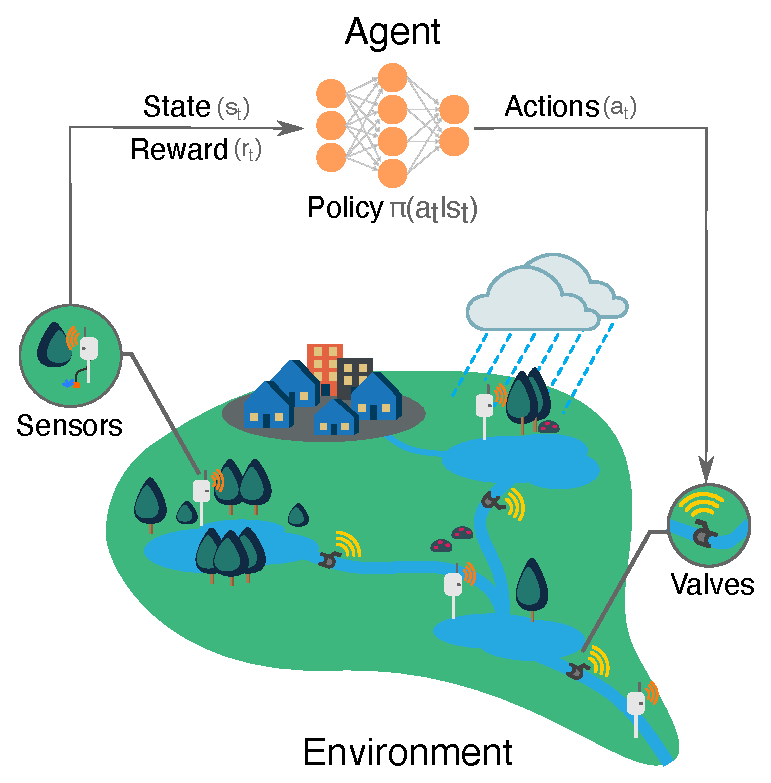
\includegraphics[width=\textwidth]{gfx/Chapter-3/RL_main_fig_1_final.eps}
    \caption{During a storm event, a reinforcement learning controller observes the state (e.g.\ water levels, flows)  of the stormwater network and coordinates the actions of the distributed control assets in real-time to achieve watershed-scale benefits.}
    \label{fig:1}
\end{figure}

Across the Artificial Intelligence and Behavioral research communities, Reinforcement Learning (RL) has emerged as a state-of-the-art methodology for autonomous control and planning systems.
Unlike in classical feedback control, where the controller carries out a pre-tuned and analytical control action, an RL controller (i.e.\ an RL agent) learns a control strategy by interacting with the system - effectively trying various control strategies until learning those that work well.
Rather than just learning one particular control strategy, an RL agent continuously attempts to improve its control strategy by assimilating new information and evaluating new control strategies \cite{Sutton98}.
RL can be used in a model free context since the system’s dynamics are implicitly learned by evaluating various control actions.
Leveraging the recent advancements in Deep Neural Networks and the computational power afforded by the high performance clusters (HPCs), RL agents have been able to plan complex tasks, such as observing pixels to play video games at a human level \cite{Mnih2015}, defeating world champions in the game of GO \cite{silver2017masteringgo}, achieving “superhuman” performance in chess \cite{Silver2017MasteringAlgorithm}, controlling high speed robots \cite{Kober2013ReinforcementSurvey}, and navigating autonomous vehicles \cite{Ng2006AutonomousLearning}.
Despite the wide adoption of Deep Neural Network based Reinforcement Learning (Deep RL) in various disciplines of engineering, its adoption in civil engineering disciplines has been limited \cite{abdulhai2003reinforcement,bhattacharya2003neural, castelletti2010tree}.
Deep RL control has yet to be applied to the real-time control of urban drainage systems.

\

Deep RL agents approximate underlying system dynamics implicitly, hence not requiring a simplified or linearized control model \cite{Sutton98}.
A Deep RL agent instantaneously identifies a control action by observing the network dynamic, thus reducing delay in the decision process \cite{Mnih2015, Silver2017MasteringAlgorithm}.
The explorative nature of the Deep RL agents also enables the methodology to adapt its control strategy to changing conditions of the system \cite{Sutton98}.
Hence, Reinforcement Learning shows promise as a potential alternative or supplement to existing control methods for water systems.
To that end, the goal of this chapter is to formulate and evaluate of Reinforcement Learning for the real-time control of urban drainage systems.
The specific contributions of the chapter are:
\begin{enumerate}
    \item The formulation and implementation of a reinforcement learning algorithm for the real-time (non-predictive) control of urban stormwater systems.
    \item An evaluation of the control algorithm under a range of storm inputs and network complexities (single stormwater basins and an entire network), as well as an equivalence analysis that compares the approach to passive infrastructure solutions.
    \item A fully open-sourced implementation of the control algorithm to promote transparency and permit for the direct application of the methods to other systems, shared on open-storm.org.
\end{enumerate}

\section{Methods}
\subsection{Reinforcement learning for stormwater systems}
When formulated as a Reinforcement Learning (RL) problem, the control of stormwater systems can be fully described by an agent and environment (figure~\ref{fig:1}).
The environment represents an urban stormwater system and the agent represents the entity controlling the system.
At any given time $t$, the agent takes a control action $a_t$ (e.g.\ opening a valve or turning on a pump) by observing any number of states $s_t$ (e.g.\ water levels or flows) in the environment.
Based on the outcomes of its action, the agent receives a reward $r_t$ from the environment.
The reward is formulated to reflect the specific control objectives.
For example, an agent could receive positive reward for preventing flooding or a negative reward for causing flooding.
By quantifying these rewards in response to various actions over time, the agent learns the control strategy that will achieve its desired objective \cite{Sutton98}.
The agent's control actions in any given state are governed by its policy $\pi$. Formally, the policy is a mapping from a given state to the agent’s actions:

\begin{equation}
    \pi :s_t (\mathbb{R}^n ) \rightarrow a_t (\mathbb{R})
\end{equation}

The primary objective of the RL control problem is to learn a policy that maximizes the total reward earned by the agent.

\

While the reward $r_t$ at the end of each control action teaches the agent the immediate desirability of taking a particular action for a given state, it does not necessarily covey any information about the long-term desirability of that action.
For many water systems, maximizing short-term rewards will not necessarily lead to the best long-term outcomes.
An agent controlling a watershed or stormwater system should have the ability to take individual actions in the context of the entire storm duration.
For example, holding water in a detention basin may initially provide high rewards since it reduces downstream flooding, but may lead to upstream flooding if a storm becomes too large.
Instead of choosing an action that maximizes the reward $r_t$  at time $t$, the agent seeks to maximize the expected long-term reward described by state-value $v$ or action-value $q$.

\

\begin{align}
	v(s_t) &= \mathbb{E} \left[\sum_{k=0}^\infty \left[\gamma^k r_{t+k+1} \Big| s_t\right] \right] \\
	q(s_t,a_t) &= \mathbb{E} \left[\sum_{k=0}^\infty \left[\gamma^k r_{t+k+1} \Big| s_t, a_t\right] \right]
\end{align}

The state-value provides an estimate for an instantaneous action, as well as potential future rewards that may arise after state $s_t$, discounted with a factor $\gamma\ (0 \leq \gamma \leq 1)$.
The action-value provides a similar estimate conditioned on taking an action $a_t$ in state $s_t$.
The discount factor $\gamma$ governs the temporal context of the reward.
For example, a $\gamma$ of 0 forces the agent to maximize the instantaneous reward, while a $\gamma$ of 1 forces it to equally weigh all the rewards it might receive for present and future outcomes.
$\gamma$ is specific to the system being controlled and can vary based on the control objective \cite{Sutton98}.

\

An RL agent can learn to control a system by learning the policy directly \cite{sutton2000policy}.
Alternatively, the agent can learn the state-value or action-value estimates and follow a policy that guides it towards the states with high estimates \cite{Sutton98}.
Several methods based on dynamic programming \cite{Watkins1992Q-learning, sutton1991planning} and Monte Carlo sampling \cite{Sutton98} have been developed to learn the functions that estimate the policy and value functions.
While these algorithms were computationally efficient and provided guarantees on the convergence, their application was limited to simple systems whose state action space can be approximated using lookup tables and linear functions \cite{Sutton98,mnih2013playing}.

\

Given the scale and the complexity of urban watersheds and stormwater networks, a simple lookup table or a linear  function cannot effectively approximate the policy or value functions for each state the agent may encounter while controlling the system.
As a simple example, considering just ten valves in a stormwater system and assuming that each valve has ten possible control actions (closed, 10\% open, 20\% open, \ldots) this gives $10^{10}$ (10 billion) possible actions that can be taken at any given state, making it computationally impossible to build an explicit lookup table for all possible states.
This, however, is where very recent advances in Deep Learning, become important.
It has been shown that, for systems with large state-action spaces, such as stormwater systems, these functions can be approximated by a Deep Neural Network  \cite{Sutton98,Mnih2015}.

\

Deep Neural Networks are a class of feed-forward artificial neural networks with large layers of interconnected neurons.
This Deeply layered structure permits the network to approximate highly complex functions \cite{hornik1989multilayer}, such as those needed for RL-based control.
Each layer in the network generates its output by processing the weighted outputs from the previous layer.
This means that each layer's output is more complex and abstract than its previous layer.
Given the emergence of cheap and powerful computational hardware over the past decade --- in particular graphical processing units (GPUs) and high performance clusters (HPCs) --- Deep Neural Networks and their variants have emerged as the state of the art in the approximation of complex functions in large state spaces \cite{LeCun2015DeepLearning}.
This makes them a good candidate for approximating the complex dynamics across stormwater systems. For purposes of this chapter, a brief mathematical summary of Deep Neural Networks is provided in SI-\ref{SI:neuralnets}.

\subsection{Deep Q Learning}

Deep reinforcement learning agents (Deep RL) use Deep Neural Networks as approximators for value or policy functions to control complex environments.
In their relatively recent and seminal Deep Q Network (DQN) chapter Mnih et al. (2015)~\cite{Mnih2015} demonstrated the first such algorithm, which used Deep Neural Networks to train an Deep RL agent to play \textit{Atari} video games at a human level.
This algorithm identifies the optimal control strategy for achieving an objective by learning a function that estimates the action values or $q$-values.
This function (i.e. $q$-function) maps a given state-action pair $(s_t,a_t)$ to the action value estimate.

\

At the beginning of the control problem, the agent does not know its environment.
This is reflected by assigning random $q$-values for all state-action pairs.
Over time, as the agent takes actions, new information obtained from the environment is used to update these initial random estimates.
After each action, the reward obtained from the environment is used to incorporate the new knowledge:

\begin{equation}
    q(s_t,a_t ) \leftarrow q(s_t,a_t ) + \alpha \left[ r_{t+1}+\gamma  \max_a q(s_{t+1},a) - q(s_t,a_t ) \right]
\end{equation}

The more actions an agent takes at any given state, the closer it gets to converging to the true action value function~\cite{Sutton98}.
The $\alpha$ (step-size) parameter governs how much weight is placed on the new knowledge~\cite{Sutton98}.

\

An agent will choose an action that maximizes its long-term reward.
This process is known as exploitation since it greedily seeks to maximize a known long-term reward.
This may not always be the best choice, however, since taking another action may lead the agent to discover a potentially better action, which it has not yet tried.
As such, the agent also needs to explore its environment.
This is accomplished by taking a random action periodically, just in case this action leads to better outcomes.
In such a formulation, the \textit{exploration vs.\ exploitation} is addressed via a $\epsilon$-greedy policy, where the agent explores for $\epsilon$ percent of time and chooses an action associated with the highest action value for the rest.
This gives the final policy for the RL agent:

\begin{equation}
    \pi(s_t) = \begin{cases}
    \text{random} \  a, & \epsilon  \\
    \underset{a}{\arg\max} \ q(s_t,a), & else
    \end{cases}
\end{equation}

$\epsilon$ is often set at a high value (e.g. 50\%) at the start of the learning process and gradually reduced to a lower value (e.g. 1\%) as the agent identifies a viable control strategy.

\

While there have been prior attempts to approximate the action value function using Deep Neural Networks, they were met with minimal success since the learning is highly unstable~\cite{Mnih2015}.
Mnih et al. (2015)~\cite{Mnih2015} addressed this by introducing a replay buffer and an additional target Neural Network.
The replay buffer acts as the RL agent’s memory, which records only its most recent experience (e.g.\ the past $10^3$ states transitions and rewards).
During the training the RL agent randomly samples data from the replay buffer, computes the neural network’s loss and updates its weights using stochastic gradient descent:


\begin{equation}
    Loss = ||\big( r_t + \gamma \max_{a'} q^* (s_{t+1},a')\big) - q(s_t,a_t) ||^2
\end{equation}

This random sampling enables the training data to be uncorrelated and has been found to improve the training process.
The target neural network  $q^*$ has the same network architecture as the main network $q$, but acts as a moving target to help stabilize the training process by reducing the variance~\cite{Mnih2015}.
Unlike the neural network approximating $q$, whose weights are constantly updated using gradient decent, $q^*$  weights are updated sporadically (e.g.\ every $10^4$ timesteps).
For more background information, Mnih et al. (2015)~\cite{Mnih2015} and Lillicrap et al.  (2016)\cite{Lillicrap2015ContinuousLearning} provide an in-depth discussion on the importance of replay memory and target neural networks in training Deep RL agents.



\subsection{Evaluation}
Here, we investigate the real-time control of urban stormwater infrastructure using Deep Reinforcement Learning.
To begin, we formulate and evaluate reward functions for the control of an individual stormwater basin.
We then extend these lessons to the control of a larger, interconnected stormwater network.
Given the relatively nascent nature of Deep RL, the need to account for public safety, and the desire to evaluate multiple control scenarios, a real-world evaluation is outside of the scope of this chapter.
As such, our analysis will be carried out in simulation as a stepping-stone toward real-world deployment in the future.
To promote transparency and broader adoption, the entire source code, examples, and implementation details of our implementation are shared freely as an open source package\footnote{\href{https://github.com/kLabUM/rl-storm-control}{https://github.com/kLabUM/rl-storm-control}}.

\

\subsection{Study Area}
\begin{figure}
    \centering
    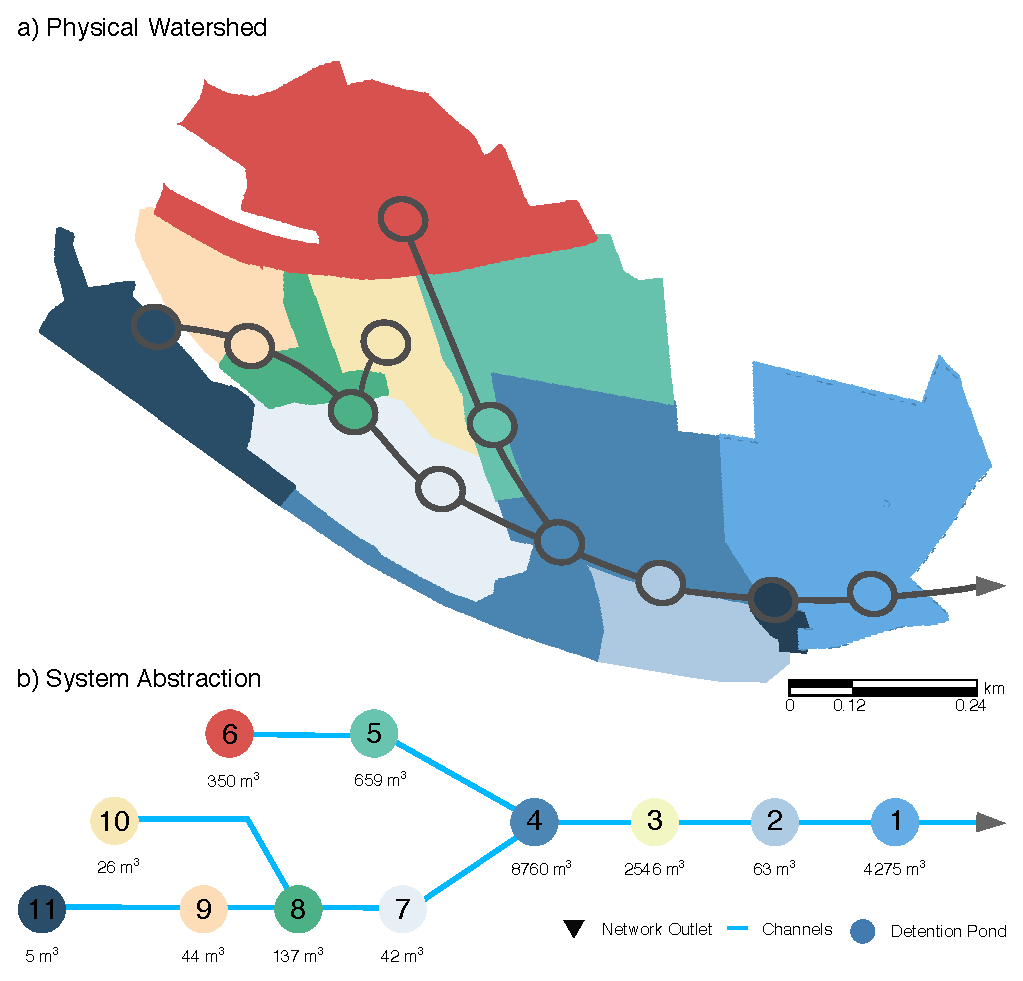
\includegraphics[width=0.7\textwidth]{gfx/Chapter-3/casestudy_fig_2.eps}
    \caption{Stormwater system being controlled in this chapter. The urban watershed includes a number of sub-catchments which drain to 11 stormwater basins of varying storage volumes. The first control scenario applies RL to the control of a single basin, while the second scenario evaluates control of multiple basins. The colors colors correspond with the catchment that contributes local runoff into each basin. Average volumes experienced by the ponds during a 25 year 6 hour storm event are presented.}\label{fig:2}
\end{figure}

Motivated by a real-world system, we apply RL control to a stormwater system inspired by an urban watershed in Ann Arbor, Michigan, USA (\ref{fig:2}). Our choice to use this watershed is motivated by the fact that it has been retrofitted by our group with wireless sensors and control valves already \cite{bartos2017open} and will, in the future, serve as a real-world testbed for the ideas proposed in this chapter. This headwater catchment features 11 interconnected stormwater basins that handle the runoff generated across $4km^2$   of predominantly urbanized and impervious sub-catchment areas.   A Stormwater Management Model (SWMM) of the watershed has been developed and calibrated in prior, peer-reviewed studies \cite{wong2018real}. It is assumed that each controlled basin in the system is equipped with a $1m^2$ square gate valve. The valves can be partially opened or closed during the simulation, which represents the action taken by an RL agent. The states of the control problem are given by the water levels and outflows at each controlled location. Given the small size of the study area, as well as the need to constrain this initial study, uniform rainfall across the study area is assumed. Groundwater base flow is assumed to be negligible, which has also been confirmed in prior studies \cite{wong2018real}.

\subsection{Analysis}
Prior Deep RL studies have revealed that performance is dependent on the formulation of reward function, quality of neural networks approximating action value function, as well as the size of state space \cite{Sutton98, henderson2017Deep}.
This creates a number of ``knobs'', whose sensitivity must be evaluated before any conclusion can be reached regarding the ability to apply Deep RL to control real stormwater systems.
As such, in this chapter, we formulate a series of experiments across two scenarios to characterize Deep RL’s ability to control stormwater systems.
In the first scenario, we control a single valve at the outlet of the watershed, comparing its particular performance under various reward function formulations.
Given that Deep RL has not been used to control water systems, this will constrain the size of the state space to establish a baseline assessment of the methodology.
In the second scenario, we scale these findings to simultaneously control multiple valves across the broader watershed and to analyze  sensitivity to function approximation (neural networks). Finally, the system-scale scenario is subjected to storm inputs of varying intensities and durations to provide broader comparison of the benefits of the controlled system in relation to the uncontrolled system.

\subsection{Scenario 1: Control of a single basin}
In this scenario, we train a Deep RL agent to control the most downstream detention basin in the network (basin 1 in figure~\ref{fig:2}).
This basin was chosen because it experiences the total runoff generated in the watershed, and because its actions have direct impact on downstream water bodies.
At any given point in time, the RL agent is permitted to set the basin’s valve to a position between fully closed or open, in 1\% increments (i.e. 0\%, 1\%, 2\%, $\ldots$, 100\% open) based on the water height in the basin. All other upstream basins remain uncontrolled.

\

The overall control objective is to keep the water height (state:$\{h_t\}$) in the basin below a flooding threshold $H_{max}$ and the outflows from the basin (state :$\{f_t\}$) below a desired downstream flooding or stream erosion threshold $F$:

\begin{align}
    h_t &\leq H_{max} \\
    f_t &\leq F
\end{align}

Three reward functions are formulated to reach this objective, each incorporating more explicit guidance (in the form of constraints) to guide the RL agent.

\

In the first reward function the RL agent receives a positive reward for maintaining the basin’s outflow below the specified threshold, a negative reward for exceeding the threshold, as well as a larger but less likely negative reward if the basin overflows:

\begin{equation}
r_1 (s_t )= \begin{cases}
		+1, & f_t \leq F\\
		-1, & f_t > F\\
		-10,& h_t > H_{max}
	\end{cases}
\end{equation}

The reward function is represented visually in the first row of figure~\ref{fig:3}.
This reward function formulation is inspired from the classic inverted pendulum problem \cite{Watkins1992Q-learning} where the agent receives +1 for success and -1 for failure.

\

The second reward function is formulated to exhibit a more complex and gradual reward structure.
In lieu of a jagged or discontinuous ``plus/minus" reward structure, the agent is rewarded for reaching flows that are close to the desired flow threshold.
It has been shown that more smooth and continuous rewards such as this, may help the agent converge onto a solution faster \cite{Sutton98, aytar2018playing}.
Visually, the reward function looks like a parabola (figure~\ref{fig:3}), where the maximum reward is achieved when the flow threshold is met exactly:

\begin{equation}
r_2 (s_t )= c_1 (f_t-c_2 )(f_t- c_3 )
\end{equation}

$c_1$, $c_2$, and $c_3$ are constants representing the scaling and inflection points of the parabola.
Here we choose $c_1$=-400 e, $c_2$=0.05, and $c_3$=0.15 to maintain the general scale of the first reward function.
Note that this formulation does not explicitly include the local constraint on the basin’s water level since the agent gets implicitly penalized by receiving a negative reward for low outflows.

\

The third reward function seeks to provide the most explicit guidance to the RL agent by embedding the most relative amount of information (third column, figure~\ref{fig:3}).
In this heuristic formulation, the agent receives the highest reward for keeping the basin empty (water levels and flows equal to zero).
Intuitively, this reward formulation seeks to drain all of the water from the basin as fast as possible without exceeding the flow and height thresholds.
If water level in the pond rises, the agent gets penalized, thus forcing it to release water.
If flows remain below the flow threshold F, the agent is penalized linearly proportional to the water level in the basin, with a more severe factor applied if the height of the basin exceeds the height threshold H. If the outflow exceeds the flow threshold F an even more severe penalty is incurred:

\begin{equation}
r_3 (s_t )= 	\begin{cases}
		c_1-c_2 h_t, & h_t < H  f_t \leq F\\
		c_1-c_3 h_t, & h_t \geq H  f_t \leq F\\
		-c_4 f_t - c_2 h_t + c_5, & h_t < H  f_t > F\\
		-c_4 f_t - c_3 h_t + c_5, & h_t \geq H  f_t > F\\
		\end{cases}
		\label{third}
\end{equation}
The penalty rates are governed by a set of five parameters c=$\{c_1,c_2,c_3,c_4,c_5\}$, which were parametrized $\{2.0, 0.25, 1.5, 10, 3\}$ to match the scales of the other two reward functions.

\

To illustrate the transferability of the control approach to variable inflows, storage volumes, and the location of a basin in the network, control by an agent trained on the third reward function is evaluated on four basins (basins 1, 4, 6, and 9 in figure~\ref{fig:2}).
These basins are chosen to represent distinct components in the network.
Basin 1 is located at the outlet of the watershed.
Basin 4 is the largest in the network and receives flows from the two major branches in the system.
Basin 6 is the largest of the upstream basins, while basin 9 is a smaller basin in series with larger basins.

\

Additionally, to analyze the performance and sensitivity of the agent to the reward function formulation, two variants of the third reward are evaluated in the supplementary information (please see SI section~\ref{SI:reward-math}) section of this chapter.
The goal of this analysis is to determine the sensitivity of the agent's performance to the choice of mathematical equations in the reward function.

\subsection{Scenario 2: Controlling multiple basins}

This scenario evaluates the ability of an agent to control multiple distributed stormwater basins.
Specifically, basins 1, 3, and 4 (figure~\ref{fig:2}) are selected for control because they experience the largest average volume during a storm event, which often corresponds with the larger control potential \cite{schutze_sewer_2008}.
It is assumed that at any time step the agent has knowledge of the water levels and valve positions for each of these basins, as well as the basin between them (basin $2$ in figure~\ref{fig:2}), thus quadrupling the number of observed states compared to the control of a single basin.
The action space must also be reduced to make the problem computationally tractable.
For the control of the single basin, there are 101 possible actions at any given time step (valve opening with 1\% granularity).
For three controlled basins, this increases to $101^3$ possible control actions at any given time step. This is not only intractable given our own computational resources, but is well beyond the size of any action space covered in other RL literature.
Here, to reduce the action space the agent is allowed to only throttle the valves. Specifically, at any time step, agent can only open or close the valve in 5\% increments or leave its position unchanged.
This results in only three possible actions for each site and thus 27 (or $3^3$) possible actions for the entire network.

\

The agent receives an individual reward for controlling each basin. These rewards are weighted equally and added together to provide a total reward for controlling the larger system. The reward for controlling each basin is given by:


\begin{equation}
	r_4 (s_t) = \begin{cases}
		-c_1 h_t+c_4, & h_t \leq H, f_t \leq F \\
		-c_2 h_t^2+c_3+c_4, & h_t > H, f_t \leq F\\
		-c_1 h_t+(F-f_t)c_5, & h_t \leq H ,f_t > F\\
		-c_2 h_t^2+c_3+(F-f_t ) c_5, &  h_t>H ,f_t>F
	\end{cases}
\end{equation}

where reward parameters  c=$\{c_1,c_2,c_3,c_4,c_5\}$ are chosen as $\{0.5,1,3,1,10\}$ to retain the relative scale of the single-basin reward formulations.
This reward seeks to accomplish practically identical objectives as the third reward function used in the single-basin control scenario.
The difference is the quadratic penalty term that is applied to the height constraint.
This modification is made to provide the agent with a more explicit guidance in response to the relatively larger state space compared to the single-basin control scenario.
In the rare instance that flooding should occur at one of the basins, agent also receives an additional penalty.

\

\subsection{Simulation, Implementation, and Evaluation}
Beyond the formulation of the reward function, the use of RL for the control of stormwater systems faces a number of non-trivial implementational challenges.
The first relates to the hydrologic and hydraulic simulation framework, which needs to support the integration of a simulation engine that is compatible with modern RL toolchains.
The second challenge relates to the implementation of the actual RL toolchain, which must include the Deep Neural Network training algorithms.

\

Most popular stormwater modeling packages, such as the Stormwater Management Model (SWMM) \cite{Rossman2010Storm5.1} and MIKE Urban \cite{Elliott2007ADrainage} are designed for event based or long-term simulation.
Namely, the model is initialized, inputs are selected, and the model run continues until the rainfall terminates or simulation times out.
While these packages support some rudimentary controls, the control logic is pre-configured and limited to simple site-scale action, such as opening a valve when level exceed a certain value.
The ability to support system-level control logic is limited, let alone the ability to interface with external control algorithms, such as the one proposed in this chapter.
To that end, we implement a step-wise co-simulation approach that was described in one of our prior studies \cite{Mullapudi2017}.

\

Our co-simulation framework separates the hydraulic solver from the control logic by halting the hydraulic model at every time step.
The states from the model (water levels, flows, etc.) are then transferred to the external control algorithm, which makes recommendation on which actions to take (valves settings, pump speeds, etc.).
Here, we adopt a python based SWMM package for simulating the stormwater network \cite{Riano-Briceno2016MatSWMMSystems}.
This allows the entire toolchain to be implemented using a high-level programming environment, without requiring any major modifications to hydraulic solvers that are often implemented in low-level programming languages and difficult to fuse with modern libraries and open source packages.
While other or more complex stormwater or hydrologic models could be substituted, model choice is not necessarily the main contribution of this chapter.
Rather, we content that SWMM adequately captures runoff and flow dynamics for the purposes of this chapter.
SWMM models the flow of water in the network using an implicit dynamic wave equation solver\cite{Rossman2010Storm5.1}.
This allows it to effectively model the nuanced conditions (e.g.\ back channel flows, flooding) that might develop in the network though real-time control.
Furthermore, the authors have access to a calibrated version of the model for this particular study area, which has been documented in a prior study \cite{aaswmm,wong2018real}.

\

One major task is the implementation of the Deep Neural Network that is used to approximate the RL agent’s action value function.
Deep Neural Networks are computationally expensive to train \cite{LeCun2015DeepLearning}.
Efficient implementation address this by leveraging a computer's graphical processing unit (GPU) to carry out this training, which is a non-trivial task.
To that end, a number of open source and community libraries have emerged, the most popular of which is \textit{TensorFlow} \cite{AbadiThisLearning}.
This state-of-the-art library has been used in some of the most well-cited RL chapters and benchmark problems, which is the reason we choose to adopt it for this study.
\textit{TensorFlow} is a python library and can be seamlessly interfaced with our python-based stormwater model implementation.

\

Multiple agents are trained and evaluated across the two scenarios: eight for the control of individual basins (across multiple reward function variants and basins), and two agents for the multi-basin control.
A Deep Neural Network is designed and implemented to learn the action-value function of each agent.
The network contains 2 layers with 50 neurons per layer.
This network is set up with a \textit{ReLu} activation function \cite{goodfellow2016Deep} in the internal layers and a linear activation function in the final layer.
The full parameters used in the study, including those for gradient descent and the DQN, are provided in the SI-\ref{SI:hyperparams} of this chapter.
A Root Mean Square Propagation (RMSprop) \cite{goodfellow2016Deep} form of stochastic gradient descent is used for updating the neural network as this variant of gradient descent has been observed to improve convergence.

\

One storm event is used to train these agents.
The SWMM model is forced with a 25-year storm event of $6\ hour$ duration and $63.5\ mm$ intensity (figure~\ref{fig:3}).
This event generates a total runoff of $3670.639\ m^3$ with a peak flow of $0.35\ m^3 /s$ at the outlet of watershed.
The agents are provided with an operational water level goal $H$ of $2\ m$, flooding level $H_{max}$ of $3.5\ m$ and outflow exceedance threshold of $F$ of $0.10\ m^3s^{-1}$.
It is important to note that the outflow threshold, in particular, serves more as an approximate guide rather than exact requirement, since the discrete valve settings used by the RL agents may not allow the exact setpoint to be physically realizable (e.g.\ throttling a valve by $5\%$ will limit outflow precision correspondingly).
These setpoints are chosen to reflect realistic flooding and stream erosion goals in the study watershed.
Agents are trained on a Tesla K20 GPUs on University of Michigan’s advanced research computing's high performance cluster.

\

The second multi-basin control agent uses the same neural network architecture of the other multi-basin RL control agent, trained this time, however, using \textit{batch normalization} \cite{ioffe2015batch}.
Batch normalization is the process of normalizing the signals between the internal layers of the neural network to minimize the internal covariance shift and has been observed to improve  the performance of the Deep RL agents \cite{Lillicrap2015ContinuousLearning}.
Ioffe et al. (2015) \cite{ioffe2015batch} provides a detailed discussion on batch normalization.

\

The performance of each agent is evaluated by comparing the RL controlled hydrographs and water levels to those that are specified in the reward functions.
For the agents controlling the individual basins, this is used to determine the importance of the reward formulation on performance, reward convergence, and training period duration.
For the multi-basin control scenario, the same approach is used to quantify overall performance, comparing this time the agent that uses the batch normalized neural network to the agent that uses the non-normalized network.

\

To evaluate the ability of an RL-agent to control storms that it is not trained on, a final analysis is carried out.
Since the agent controlling multiple basins presents the most complex of the scenarios, it is first trained on one of storms and evaluated on a spectrum of storm events with varying return periods (1 to 100 years) and durations (5 min to 24 hours).
These storm events are generated based on the SCS type II curve and historical rainfall intensities for the study region \cite{scs1986urban}.
The performance of the agent across these 70 storms is compared to the uncontrolled system to evaluate the boarder benefits of real-time control.
For comparison with an other control algorithm, we also implement and compare the performance of RL to an \textit{Equal Filling Degree} controller, which seeks to control the volume in each basin to achieve equal relative filling \cite{schutze_astlingen_2018}. Implementation details of the equal filling algorithm can be found in the SI-\ref{SI:equalfill}.
We also evaluate the performance of the RL controller on a back-to-back storm event (3 hour 5 year event, followed by a 2 hour 2 year event).
To allow for a comparison between the controlled and uncontrolled system, a non-negative performance metric is introduced to capture the magnitude and time that the system deviates from desired water level and flows thresholds.
Specifically, across a duration $T$ the final performance $P$ adds together the deviation of all $N$ controlled sites from their desired water level ($P_h$) and flow thresholds ($P_f$), where:


\begin{align}
	P_h(h) &= \begin{cases}h-H, & h>H \\ h-H+100h,  &h>H_{max} \\0, & otherwise\end{cases} \\
	P_f(f) &= \begin{cases}10(f -F), & f>F \\0, & otherwise\end{cases} \\
	P &= \sum_{n=1}^N \sum_{i=0}^T P_h (h_i^n ) + P_f (f_i^n ) \label{perf_met}
\end{align}
A relatively lower performance value is more desirable, since it implies that the system is not flooding, nor exceeding desired flow thresholds.

\section{Results}

\subsection{Scenario 1: Control of single basin}

\begin{figure}
    \centering
    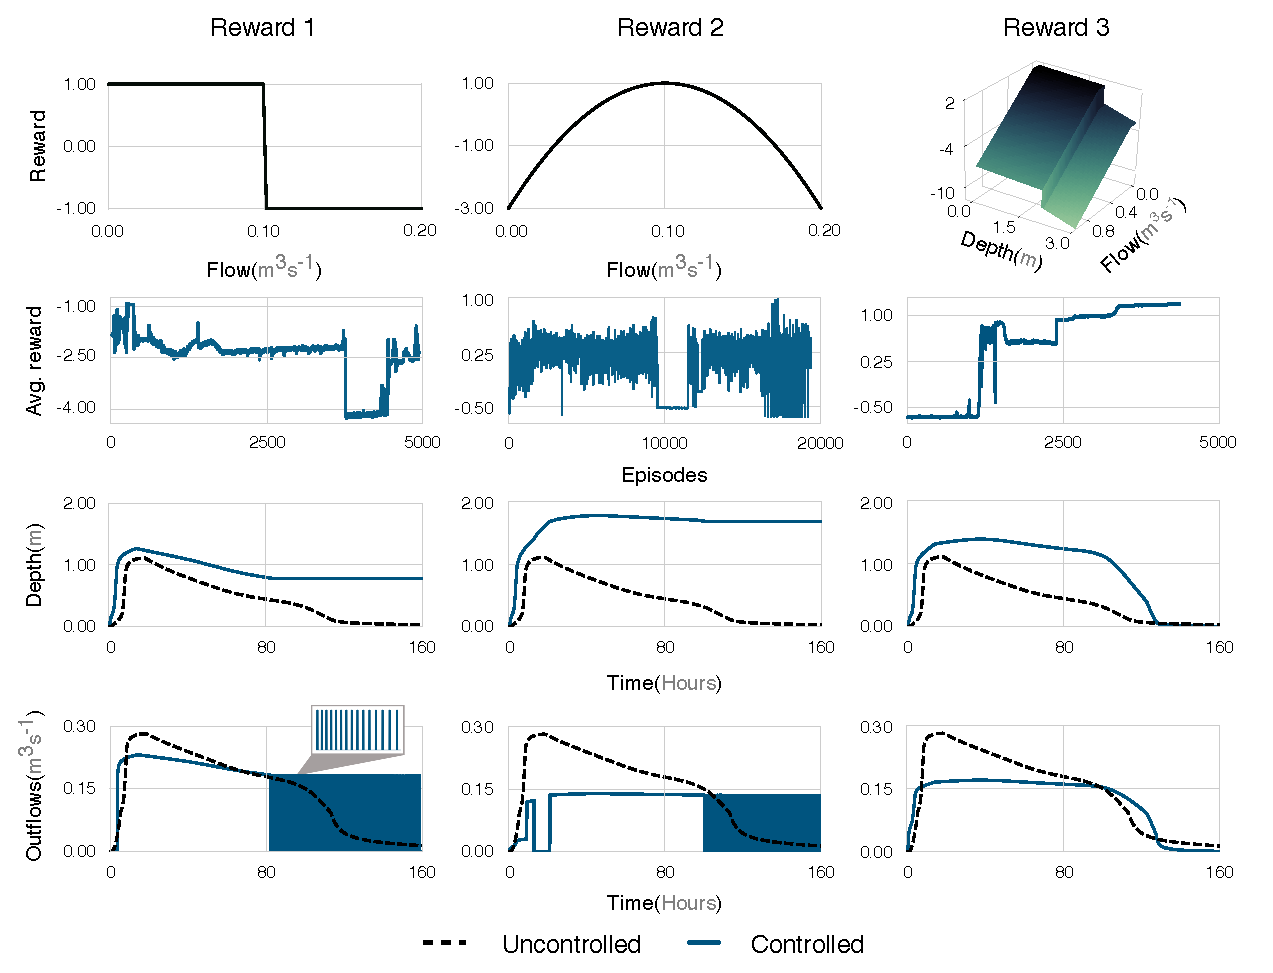
\includegraphics[width=\textwidth]{gfx/Chapter-3/single_pond.eps}
    \caption{RL control of a single basin, trained using three reward formations (grouped by column). The first row plots each reward function used during training. The second row plots the average reward received during training (please note that the scale of Y-axis differers for each reward function). The third and fourth rows compare the controlled flows and water levels with the uncontrolled, for the episode that resulted in the highest reward. Generally, reward function formulations with more explicit guidance lead to relatively better control performance and improved convergence during raining. Agents trained using relatively simple reward also exhibit a rapidly-changing and unstable control behavior, shown as a close up in the bottom left plot.}\label{fig:3}
\end{figure}



The ability of an RL agent to control a stormwater basin is highly sensitive to the reward function formulation.
Generally, a more complex reward function -- one that embeds more information and explicit guidance -- performs better, as illustrated in figure~\ref{fig:3}.
Each column of the figure corresponds with an individual RL agent, each of which is trained using a different reward function $(r_1,r_2,r_3)$.
The reward functions are plotted in the first row, while the reward received during training is plotted in the second row.
The training period is quantified in terms of episodes, each of which corresponds to one full SWMM simulation across an entire storm.
The third and fourth rows in the figure compare the uncontrolled flows and water levels, respectively, for the episode that resulted in the highest reward.

\

The RL agent that uses the simplest reward function has the relatively worst performance (figure~\ref{fig:3}, first column).
Even after 5000 training episodes (a week of real-world simulation time), the mean reward does not converge to a stable value.
Playing back the episode that resulted in the highest reward (figure~\ref{fig:3}, rows 3-4, column 1), reveals that the RL agent does retain more water than would have been held in the uncontrolled basin.
While this lowers the peak flows relative to the uncontrolled basin, the RL agent is generally not able to keep flows below the desired threshold.
More importantly, the RL agent's control actions begin oscillating and become unstable toward the middle of the simulation.
In this episode, the agent keeps the water level in the basin relatively constant by opening the valve very briefly to release just a small amount of water.
This “chattering” behavior (shown as a close up in the figure) results in an unstable outflow pattern that oscillates in a step-wise fashion between $0\ m^3/s$ and $0.18\ m^3/s$.
For various practical reasons, such rapid control actions are not desirable.
Since the RL agent never once receives a positive reward, it may have converged onto an undesirable local minimum during the training.
Providing more time for training does not appear to resolve this issue, which may also suggest that a stable solution cannot be derived using this particular reward formulation.

\

Embedding more explicit guidance (harder constraints) into the reward formulation improves the control performance of the RL agent (figure~\ref{fig:3}, second column).
When the second and more continuous reward function is used by the agent, the highest reward episode reveals that the RL agent is relatively more effective at maintaining flows at a constant value.
Unlike the RL agent using the simple step-wise reward function, the RL agent using the parabolic reward function has more opportunities to receive smaller, more gradual rewards.
During most of the episode, this increased flexibility allows the second RL agent to receive positive rewards and keep the outflow below a flow threshold of $0.14\ m^3/s$.
While relatively improved, the RL agent using the parabolic reward also does not converge to a stable reward value.
However, toward the end of the episode, this RL agent also carries out irregular and sudden control actions by opening and closing the valve in short bursts.
In this case, the RL agent is oscillating between a maximum (valve open) and minimum (valve closed) reward rather than taking advantage of variable rewards in other configurations.
This suggests that the agent has either not yet learned a better strategy or, again, that a stable solution cannot be converged upon using this particular reward formulation.
This speaks to the need for more explicit constraints as well, since a real-world stormwater system could not be throttled in this fashion. Simply put, the reward formulations used in this case was too simple to achieve realistically desirable outcomes.

\

The RL agent using the third and most constrained formulation exhibits the relatively best control performance.
This agent regulates flow and water levels in a relatively gradual and smooth manner.
Unlike in the case of the other two RL agents, after 3500 training episodes, the third agent does converge to a steady reward.
Evaluating the episode resulting in the highest reward (figure~\ref{fig:3}, rows 3-4, column 3), the desired “flat” outflow hydrograph is achieved.
No unstable or oscillatory control actions are evident, as in the case of the other two reward functions.
The agent is able to maintain flows below a constant threshold of $0.15\ m^3/s$.
While this is not the exact threshold that was specified ($0.1\ m^3/s$), it is close considering that the achievable threshold is dependent on water levels and the ability to only throttle the valve in 1\% increments.
As stated in the methods section, matching the exact threshold may not be physically realizable in any given situation due to constraints enforced by discretized throttling.
Furthermore, the RL agent must balance the desired outflow against the possibility of flooding and is thus more likely to release a greater amount of water than is specified by the threshold. Interestingly, this agent does not change its valve configuration at all.
Rather, it keeps its valve 54\% open the entire time of the simulation, which allows it to meet a mostly constant outflow given the specific inflows. Overall, the general shape of the outflows is improved compared to the uncontrolled scenario.
Furthermore, an added benefit of real-time control is that the overall volume of water leaving the basin is also reduced by 50\% due to infiltration.

\

Similar to the third reward function, agents trained on the 3a and 3b reward functions are successfully able to maintain the outflows close to the threshold during the stormevent (figure~\ref{fig:new_reward_math} in SI~\ref{SI:reward-math}).
While these reward functions may appear similar, the solution identified by their respective agents differs.
This is a result of the difference between the decay rates in the exponential and squared terms.
Performance of the agent trained on the 3a and 3b reward functions (SI~\ref{SI:reward-math}) indicates that the ability of the agent to identify a viable control strategy is not dependent on the choice of equations used for the creating the reward functions, but rather on the  general shape of the reward function in the domain.

\

The agent using the third reward function (trained on basin 1), is able to control basins 4,6 and 9 without any further modifications (SI~\ref{SI:reward-loc}, figure~\ref{fig:9}).
The agent in this formulation makes its control decisions only based on the depth at the current time step and does not incorporate any predictions.
Hence, the ability of the controller to shape of outflows should not dependent on the location of the basin in the network, magnitude of inflows or the storage curves.
Our simulation results indicate the same.
Though the degree to which the agent is able to achieve the objective is governed by these physical constraints, its ability to discover a solution is not influenced by them.

\

This scenario, which focuses on the control of a single site, emphasizes the importance of the reward function formulation in RL-based control of stormwater systems.
The complexity of the reward formulation plays an important role in allowing the RL agent to learn a control policy to meet the desired hydrologic outcomes.
The importance of reward formulations has been acknowledged in prior studies\cite{Sutton98, ng1999policy}.
Generally, reward functions with more explicit guidance lead to a more rapid convergence of a control policy, while avoiding unintended control actions, such as the chattering behavior seen in figure~\ref{fig:3}.
In fact, prior studies have attributed such erratic control actions to the use of oversimplified reward functions \cite{ng1999policy}, but have offered little specificity or concrete design recommendations that could be used to avoid such actions.
As such, our approach heuristically evaluates reward formulations of increasing complexity until arriving at one that mostly meets desired outcomes.
This introduces an element of design into the use of RL for the real-time control of stormwater, as one cannot simply rely on the implicit black box nature of neural networks to solve a control problem under complex system dynamics.
The reward function needs to embed enough information to help guide the RL agent to a stable solution.
This introduces only a limited amount of overhead, as reward functions can be intuitively formulated by someone with knowledge of basic hydrology.

\

For control of individual basins, the reward function presented here should be directly transferable.
If more complex outcomes are desired, modifications to the reward function may need to be carried out.
Objectively, the convergence of the reward will serve as one quality measure of control performance.
The ultimate performance of RL for the control of individual sites will, however, need to be assessed on a case-by-case basis by a designer familiar with the application.
Taking the baseline lessons learned during the control of a single basin, the second scenario can now evaluate the simultaneous control of multiple basins.

\subsection{Scenario 2: Control of multiple basins}

\begin{figure}
    \centering
    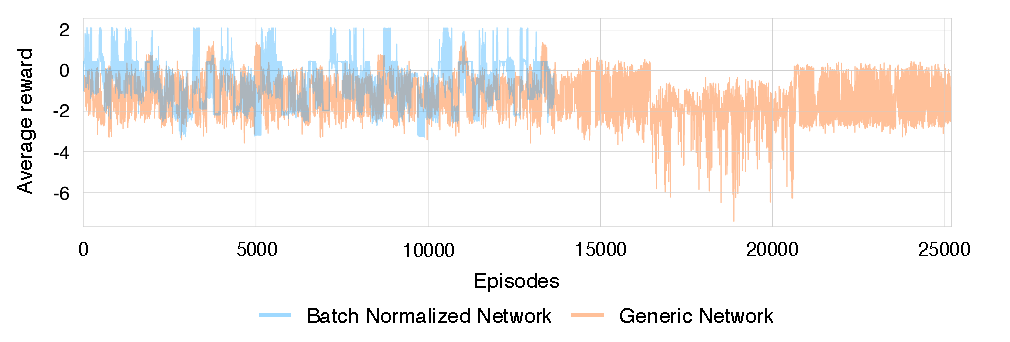
\includegraphics[width=\textwidth]{gfx/Chapter-3/system_tarining.eps}
    \caption{Average reward earned by the RL agent when learning to control multiple basins. The use of neural network batch normalization (blue) leads to consistently higher rewards when compared to the use of a generic neural network (orange).  The batch normalized network also leads to higher rewards earlier in the training process.}
    \label{fig:4}
\end{figure}


When trained using the generic feed forward neural network configuration that was used for the control of a single basin, the RL agent controlling multiple assets was unable to converge to a stable reward, even after 25000 episodes of training (figure~\ref{fig:4}).
This totaled to $\approx$52 days of computation time on our GPU cluster, after which the training procedure was halted due to lack of improved reward.
Overall, learning performance was low in this configuration.
Not only did the learning procedure not converge to a stable reward, but the vast majority of rewards were negative.
Given this observation, this ineffective neural network was then replaced with one that was batch normalized.
The agent using the batch normalized neural network achieved a higher average reward than the agent with a generic feed forward neural network (figure~\ref{fig:4}).
Furthermore, the agent using the batch normalized neural network achieved a relatively high rewards early on in the training process, thus making it more computationally favorable.
While beyond the scope of this study, this suggests that the choice of neural network architecture is likely a major design factor in the successful implementation of RL-based stormwater control.

\

Even with batch normalization, the RL agent did not consistently return to the same reward or improve its performance when perturbed.
The exploration in its policy caused the RL agent to oscillate between local reward maxima.
Similar outcomes have been observed in a number of RL benchmark problems\cite{henderson2017Deep, Mnih2015}, which exhibited a high degree of sensitivity to their exploration policy.
Prior studies have noted that the exploration-exploitation balance is difficult to parameterize because neural networks tend to latch onto a local optimum \cite{larochelle2009exploring}.
As such, it is likely that the lack of convergence observed in this scenario was caused by the use of a neural network as a function approximator.
Forcing neural networks to escape local minima is still an ongoing problem of research~\cite{osband2016Deep}.
Nonetheless, even without a consistent optimum, the maximum reward obtained during this scenario can still be used as part of an effective control approach.

\


\begin{figure}
    \centering
        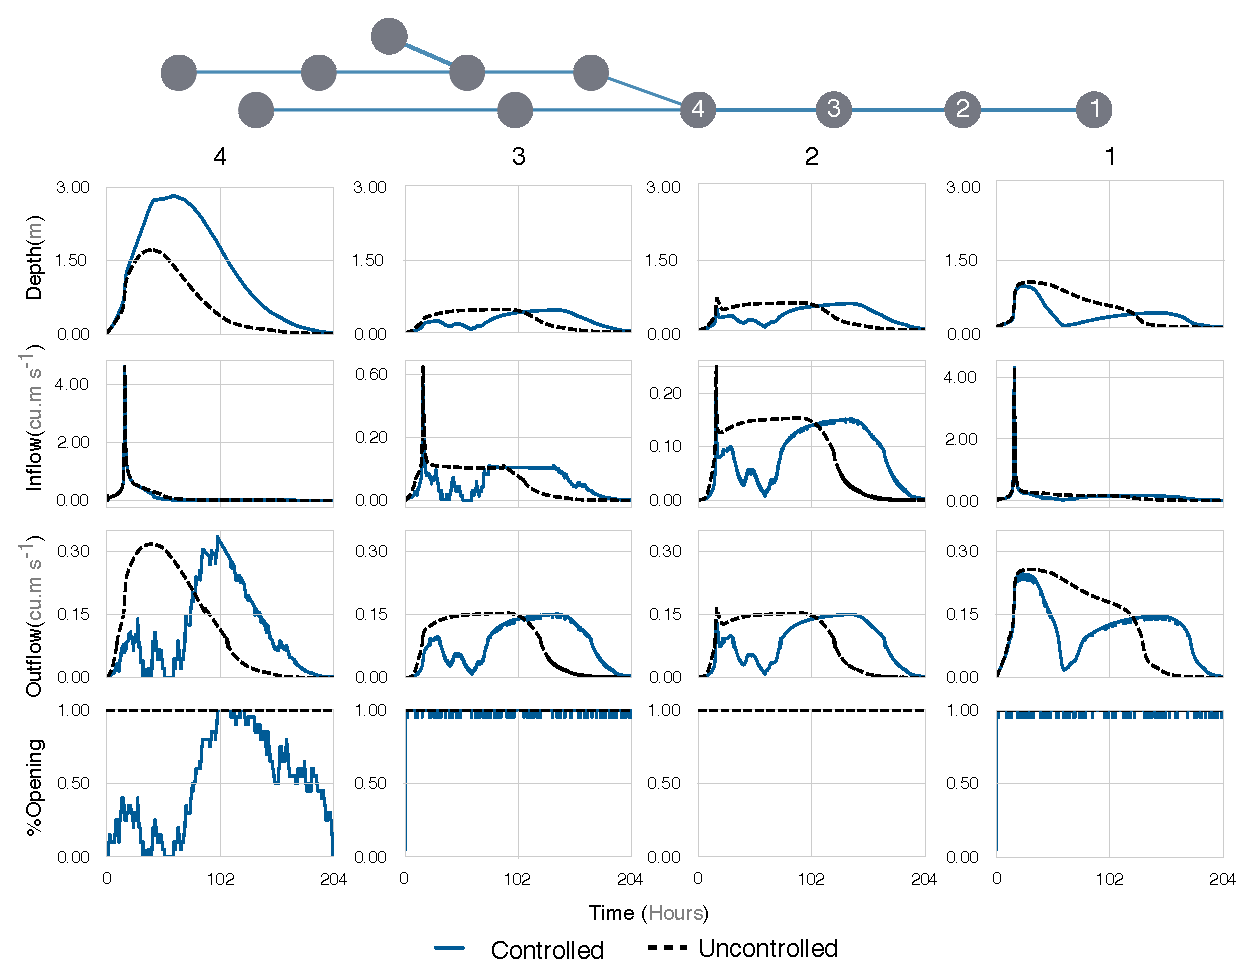
\includegraphics[width=\textwidth]{gfx/Chapter-3/system_scale_1.eps}
    \caption{RL agent controlling multiple stormwater basins during a 6-hour, 25-year storm event. Control actions at each of the controlled basins are shown as valve settings in the fourth row of the plot. In this scenario, the agent achieves a high reward by just controlling the most upstream control asset (4) and shifting the peak of the hydrograph. Difference in the scale of Y-axis in second row demonstrates the wide range of inflows in the network.}\label{fig:ch3-fig5}
\end{figure}

Selecting the episode with the highest reward revealed the actions taken by the RL agent during the training storm (figure~\ref{fig:ch3-fig5}).
The figure compares the controlled and uncontrolled states of the four basins during a 25-year 6-hour storm event, showing the depth in each basin, inflows, outflows, and control actions taken by the RL agent.
Though basin 2 is not explicitly controlled by the controller, given that the water level and outflows in this basin are impacted by the actions taken in the upstream basin, we have chosen to present its response.
No flooding occurred during this simulation, which means that the reward received by the RL agent was entirely obtained by meeting outflow objectives.
The valves on basins 1 and 3 throttled between 100\% and 95\% open, which for all practical considerations could be considered uncontrolled.
As such, the RL agent in this scenario earned its reward by only controlling the most upstream basin in this network.

\

While the outcome of control was somewhat favorable compared to the uncontrolled systems, the playback of the highest reward in figure~\ref{fig:ch3-fig5} does not show drastically different outcomes.
Control of the $4^{th}$ basin shifted the timing of the outflows from the basin but did not reduce its outflows.
This resulted in improvements at the $1^{st}$, $2^{nd}$ and $3^{rd}$ basins.
By delaying flows from the $4^{th}$ basin, the RL agent allowed the downstream basins to drain first and to spend less time exceeding the flow threshold.
Interestingly, the RL agent did not control basin 1, even while the single-basin control scenario makes it is clear that a more favorable outcome can be achieved with control (figure~\ref{fig:3}).
As such, a better control solution may exist, but converging to such a solution using a neural network approximator is difficult.
This likely has to do with the larger state action space.
While the site-scale RL agent was only observing water level at one basin, the system level RL agent had to track levels and flows across more basins, which increases the complexity of the learning problem.
The rewards received by the RL agent in the scenario are cumulative, which means that improvement at just a few sites can lead to better rewards, without the need to control all of them.
Increasing the opportunity to obtain rewards thus increases the occurrence of local minima during the learning phase.

\

In the single basin control scenario, the RL agent can immediately observe the impact of its control actions.
In the system scale scenario more time is needed to observe water flows through the broader system, which means that the impact of a control action may not be observed until later timesteps.
This introduces a challenge, as the RL agent has to learn the temporal dynamics of the system.
This challenge has been observed in other RL studies, which have shown better performance for reactive RL problems, as opposed to those that are based on the need to plan for future outcomes \cite{aytar2018playing}.
The need to include planning is still an active area of RL research.
Potential emerging solutions include adversarial play\cite{silver2017masteringgo,Silver2017MasteringAlgorithm}, model-based RL\cite{clavera2018model}, and policy-based learning \cite{Schulman2017ProximalAlgorithms}.
The benefits of these approaches have recently been demonstrated for other application domains and should be considered in the future for the control of water systems.

\

\begin{figure}
    \centering
    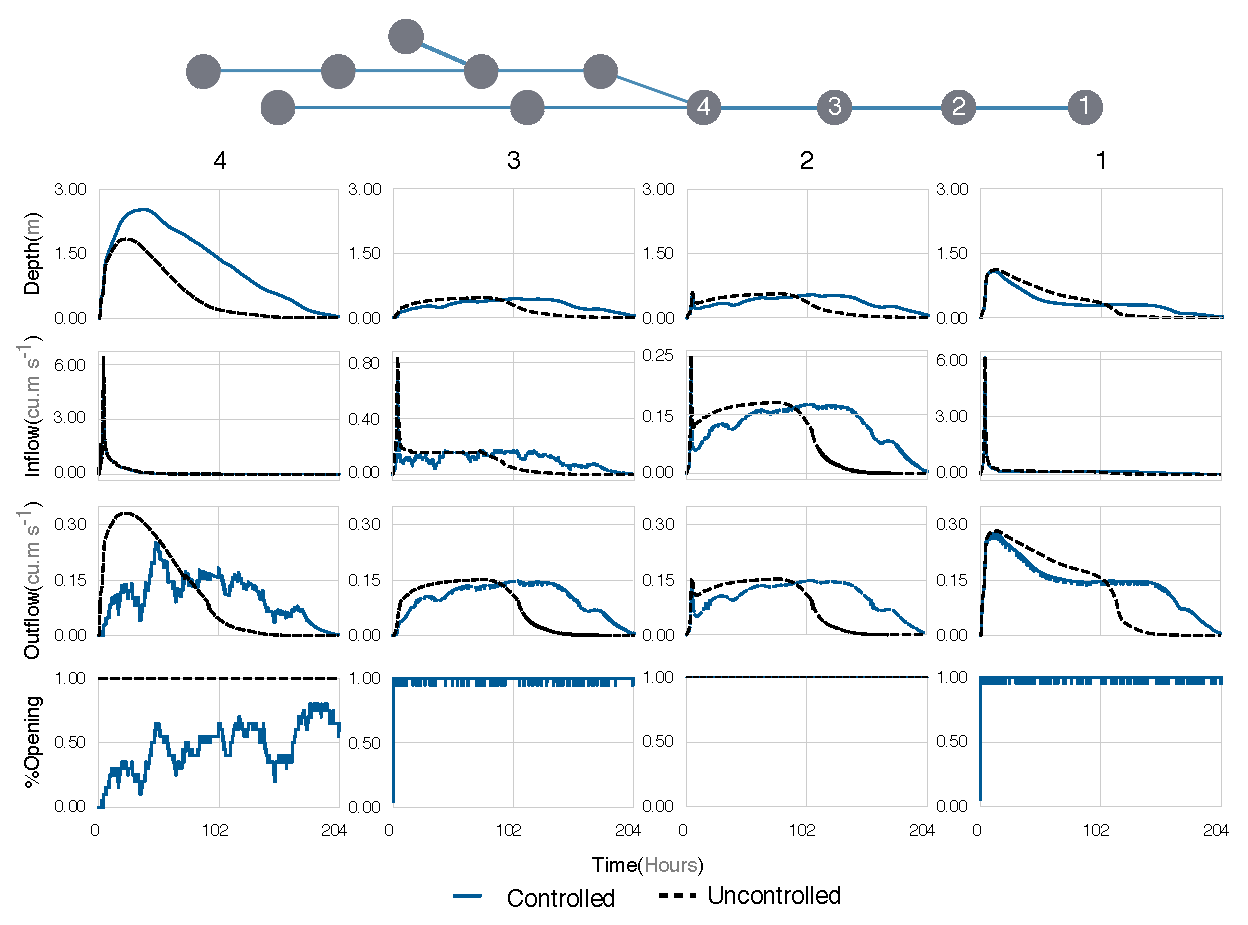
\includegraphics[width=\textwidth]{gfx/Chapter-3/system_scale_2.eps}
    \caption{RL agent controlling multiple stormwater basins during a 24-hour, 10-year storm event. Control actions at each of the controlled basins are shown as valve settings in the fourth row of the plot. In this scenario, the agent achieves a high reward, by maximizing the storage utilization in the most upstream control asset (4) and regulating the outflow from it to meet the downstream objectives. Difference in the scale of Y-axis in second row demonstrates the wide range of inflows in the network.}\label{fig:ch3-fig6}
\end{figure}

It is important to note that figure~\ref{fig:ch3-fig5} represents an evaluation of the RL agent for one storm only – namely, the training storm.
Realistically, the control system will need to respond to storms of varying durations and magnitudes.
As an example, the RL agent’s response to a 24-hour, 10-year storm is shown in figure~\ref{fig:ch3-fig6}.
Performance of the controller in controlling a back-to-back event is presented in SI-\ref{SI:b2b-events}.
Here, the RL agent outperformed the uncontrolled system much more notably compared to the training storm.
The controlled outflows were much closer to the desired threshold, even when only one basin was controlled.
This broader performance is captured in figure~\ref{fig:ch3-fig7}, which quantifies performance (eq.~\ref{perf_met}) across a spectrum of storm inputs.
Figure~\ref{fig:ch3-fig7} compares the uncontrolled system to the RL-controlled system.
Both the controlled  and uncontrolled systems perform equally well during small-magnitude and short events (e.g.\ the training storm in figure~\ref{fig:ch3-fig5}).
The benefits of control become more pronounced for larger events, starting at 10-year storms and those that last over 2 hours.
This visualization holistically captures the benefits of real-time control by highlighting new regions of performance and showing how control can push existing infrastructure to perform beyond its original design.

\

\begin{figure}
    \centering
    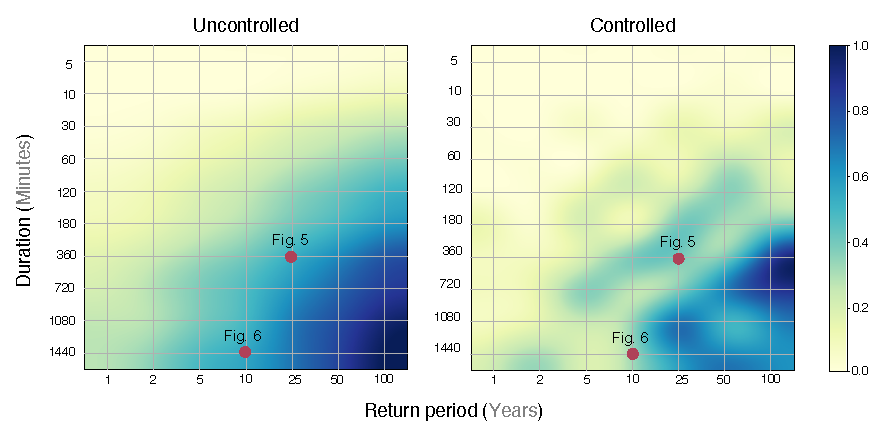
\includegraphics[width=\linewidth]{gfx/Chapter-3/heatmap.eps}
    \caption{Normalized performance of stormwater system (eq.~\ref{perf_met}) for the uncontrolled system (left) and RL-controlled system (right). The use of control enhances the performance stormwater network by allowing the system to achieve desired outcomes across larger and longer storms. The lighter color (closer to zero) corresponds with a relatively better performance.}\label{fig:ch3-fig7}
\end{figure}


\section{Discussion}

Given the recent emergence and popularity of Reinforcement Learning, much research still remains to be conducted to evaluate its potential to serve as a viable methodology for the RTC of water systems.
Our study brings to light a number of benefits and challenges associated with this task.
Arguably, it seems that the major benefit of using RL to control water systems is the ability to simply hand the learning problem to a computer without needing to worry about the many complexities, non-linearities and formulations that often complicate other control approaches.
However, as this study showed, this comes with a number of considerable caveats.
These include the challenges associated with formulating rewards, choosing function approximators, deciding on the complexity of the control problem, as well as contending with practical implementation details.

\

Our study confirms that the performance of RL-based stormwater control is sensitive to the formulation of the reward function, which has also been observed in other application domains~\cite{ng1999policy}.
The formulation of the reward function requires domain expertise and an element of subjectivity, since the RL agent has to be given guidance on what constitutes appropriate actions.
In the first scenario, it was shown that a reward function that is too simple may lead to adverse behavior, such as the chattering or sudden actions.
The reward may also not converge to a stable solution since the neural network can take advantage of the simple objective to maximize rewards using sudden or unintuitive actions.
The formulation of the problem, which depends heavily on neural networks, also makes it difficult to determine why one specific reward function may work better than another.
Increasing the complexity of the reward function, by incorporating more explicit guidance, was shown to help guide the RL agent to a more desirable outcome. In other control approaches, such as genetic algorithms or model predictive control, the design of reward is an iterative process, and sometimes involves anticipating fringe cases to improve the robustness of the controller.
Similar to these approaches, we can however begin using this early study to formulate a number of practical considerations when formulating reward functions:
\begin{itemize}
    \item Define the reward function for entire domain of the state-action space, ensuring that it distinguishes the desirable actions from the undesirable ones.
    \item Ensure that the reward function represents a specific hydrologic response that the controller is to achieve, while anticipating, as much as possible, alternate and adverse  hydrologic responses that the controller may discover to maximize the reward function.
    \item Relax the mathematical formulation of the reward function and focus rather on the two above points (e.g.\ the shape of a reward surface rather than its specific mathematical form).
\end{itemize}
Reward formulations are an ongoing research area in the RL community and some formal methods have recently been proposed to provide a more rigorous framework for reward synthesis~\cite{fu2017learning}. These formulations should be investigated in the future.


\

Even when the choice of reward function is appropriate or justifiable, the control performance can become sensitive to the approximation function, which in our case took the form of a Deep Neural Network.
Choosing the architecture and structure of the underlying network becomes an application dependent task and can often only be derived through trial and error~\cite{Sutton98, henderson2017Deep}.
Secondly, for challenging control problems, such as the one studied here, learning the mapping between rewards and all possible control decisions becomes a complex task.
The neural network must be exposed to as many inputs and outputs as possible, which is computationally demanding.
In our study we ran simulations for many real-world months on a high performance cluster, but it appears that the learning phase could have continued even longer.
This, in fact, has been the approach of many successful studies in the RL community, where the number of computers and graphical processing units can be in the hundreds~\cite{espeholt2018impala, OpenAI_dota}.
This was not feasible given our own resources, but could be evaluated in the future.

\

Aside from the formulation of the learning functions and framework, the actual complexity and objectives of the control problem may pose a barrier to implementation.
We showed that an RL agent can learn how to control a single stormwater basin effectively, but that controlling many sites at the same time is difficult.
A major reason is the increase in the number of states and actions that must be represented using the neural network.
While computational time may remedy this concern, the structure of the neural network may also need to be altered.
In a system-scale stormwater scenario, actions at one location may influence another location at a later time.
As such, the agent would benefit from a planning-based approach which considered not only current states, but future forecasts as well.
Such planning-based approaches have been proposed in the RL literature and should be investigated to determine if they lead to an improvement in performance~\cite{clavera2018model,depeweg2016learning}.
Furthermore, model-based approaches have also recently been introduced and could allow some elements of the neural network to be replaced with an actual physical or numerical stormwater model~\cite{gu2016continuous}.
Such approaches should be evaluated in the future since they may permit more domain knowledge from water resources to be embedded into training the controller.

\

It is important to note that the Equal-filling algorithm outperforms the RL agent in this study (SI-\ref{SI:equalfill}).
It achieves the objective of maintaining the outflow below the desired threshold without causing flooding.
Since Equal-filling outperforms RL, it could very well be considered a superior choice in this study.
That said, developing and deploying Equal-filling often requires an intuitive understanding of the system and require a highly manual tuning of parameters.
While it may be relatively straightforward to design control approaches in smaller systems and simple outcomes ---such as the one in this study --- developing coordinated control strategies for large scale systems with multiple-objective might not be as easy.
As such, we see RL-based control as a long-term goal, which should be investigated in future studies across bigger scales and complex outcomes.
Our study presents an initial goal toward the broader study of RL-based stormwater control, after which an comprehensive apples-to-apples comparison may be possible with current state-of-the-art approaches.

\

Finally, the use of RL for the control of stormwater systems is underpinned by a number of practical challenges.
Computational demands are very high, especially compared to competing approaches, such as dynamical systems control, model predictive control, or market-based controls.
While computational resources are becoming cheaper, the resources require to carry out this study were quite significant and time demanding.
Since actions taken by neural networks cannot easily be explained and explicit guarantees cannot be provided, this may limit adoption by decision makers who may consider the approach a “black box”.
It is also unlikely that the control of real-world stormwater systems will simply be handed over to a computer that learns through mistakes.
Rather, simulation-based scenarios will be required first.
It has recently been shown as long as a realistic simulator is used --- in our case SWMM --- then the agent can be effectively trained in a virtual environment before refining its strategy in the real world~\cite{OpenAI_dota}.

\section{Conclusion}

This chapter introduced an algorithm for the real-time control of urban drain\-age systems based on Reinforcement Learning (RL).
While RL has been used successfully in the computer science communities, to our knowledge this is the first instance for which it has been explicitly adopted for the real-time control of urban water systems.
The methodology and our implementation show promise for using RL as an automated tool-chain to learn control rules for simple storage assets, such as individual storage basin.
However, the use of RL for more complex system topologies faces a number of challenges, as laid out in the discussion.
Simultaneously controlling multiple distributed stormwater assets across large urban areas is a non-trivial problem, regardless of the control methodology.
To that end, the concepts, initial results and formulations provided by this chapter should help build a foundation to support RL as a viable option for stormwater control.
The source code accompanying this chapter should also allow others to evaluate many other possible architectures and parameterizations that could be used to improve the results presented in the chapter.
